\chapter{Time Travel Functionality}
\label{ch:timetravel}

%\epigraph{%
%    Marty McFly: Wait a minute, Doc. Are you telling me that you built a time machine\ldots out of a Postgres server?
%	
%    Dr. Emmett Brown: The way I see it, if you're gonna build a time machine, why not do it in style?
%}{Back to the Future I}

In this Chapter, the various concepts regarding the so called \emph{time travel} functionality, how it pertains the presented CDC system, and the issues that arose in implementing this feature, will be discussed.
Additionally, some background to this functionality will be presented in the following Section.

%Let us begin the discussion of this feature.
A time traveled table is a table in the output database that holds the information of present and past states of its source table.
Let us introduce a time travel operator $\tau$, so that for some table $\omega$, similarly to the previous Chapter \ref{ch:data}, we can write
$$
\dest{\omega} := \tau(\source{\omega}) \; .
$$

Before giving a definition of $\tau$, further notation is required.

Let us indicate with $r_i$ a particular configuration of some row $r$'s values, which belongs to table $\omega$, such that $r$, identified by its primary key, is updated in $\source{\omega}$ from $r_i$ to $r_{i + 1}$.
This change of values must happen at a particular moment, thus let a data change record $r_i^t$ convey update number $i$ to $r$'s values, emitted at time $t$.

In Figure \ref{fig:tt-intro} a visual representation of the above notation is portrayed.
In particular, $r_0$ is the configuration of $r$'s values at insertion time $t$, while the following are those configurations that $r$ acquires, at successive updates.

\begin{figure}
	\centering
	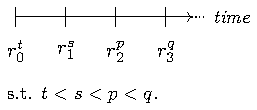
\includegraphics[width=0.4\linewidth]{figures/time-travel/intro}
	\caption{Representation of changes to a row $r$.}
	\label{fig:tt-intro}
\end{figure}

With this notation, a definition of $\tau$ is possible.

\begin{definition}[Time travel operator]\label{def:tau}
	Whichever attributes is $\source{\omega}$'s primary key composed of, it is extended, in $\dest{\omega}$, to contain a validity range; that is, the range of time in which some configuration $r_i$ of $\source{\omega}$'s row $r$ was the configuration that could be retrieved from the source database, when reading $r$; $\forall r \in \source{\omega}$.
\end{definition}

This validity range is expressed as a numerical range of the form $[x, y)$, such that $x, y \in T$, where $T$ is the totally ordered set of all instants of time, present and past.
For our purposes, let us say that $\pm\infty \in T$, so that a range of the form $[x, +\infty)$ is intended to mean that some configuration $r_i$ is valid from instant $x$ up to an unknown moment in the future, and a range of the form $(-\infty, x)$ is intended to mean that a validity ends at instant $x$.

\begin{example}
	To accomplish the changes depicted in Figure \ref{fig:tt-intro}, the resulting validity data in $\dest{\omega}$ can be expressed as in Table \ref{tab:tt-validity}.
	Note how receiving an update causes the old configuration to be retained, and to have its validity range updated.
\end{example}

\begin{table}
	\centering
	\begin{tabular}{cc}
		$r$ & \emph{validity} \\
		\hline
		$0$ & $[t, +\infty)$ \\
	\end{tabular}
	\hspace{1mm}
	\begin{tabular}{cc}
		$r$ & \emph{validity} \\
		\hline
		$0$ & $[t, s)$ \\
		$1$ & $[s, +\infty)$ \\
	\end{tabular}
	\hspace{1mm}
	\begin{tabular}{cc}
		$r$ & \emph{validity} \\
		\hline
		$0$ & $[t, s)$ \\
		$1$ & $[s, p)$ \\
		$2$ & $[p, +\infty)$ \\
	\end{tabular}
	\hspace{1mm}
	\begin{tabular}{cc}
		$r$ & \emph{validity} \\
		\hline
		$0$ & $[t, s)$ \\
		$1$ & $[s, p)$ \\
		$2$ & $[p, q)$ \\
		$3$ & $[q, +\infty)$ \\
	\end{tabular}
	\caption{Representation in $\dest{\omega}$ of the changes outlined in Figure \ref{fig:tt-intro}.}
	\label{tab:tt-validity}
\end{table}

Let us now draw an algorithm with which operations on the source table are mapped, using time travel logic, to operations in the output database.
We do so, by defining the following Operations (\ref{tt:insert}), (\ref{tt:update}), and (\ref{tt:delete}), which exhaustively comprise all relevant classes of data change events.

\begin{equation}\label{tt:insert}
	\source{\omega} \rightarrow \text{\texttt{INSERT} } r_i^t \xRightarrow{\tau}
	\text{\texttt{INSERT} } r_i \text{ s.t. } \text{validity} := [t, +\infty)
\end{equation}

\begin{equation}\label{tt:update}
	\source{\omega} \rightarrow \text{\texttt{UPDATE} } r_i^t \xRightarrow{\tau}
	\begin{Bmatrix}
		\text{1. \texttt{UPDATE} } r_{i-1} \text{ s.t. } \text{validity} \cap (-\infty, t) \\
		\text{2. \texttt{INSERT} } r_i \text{ s.t. } \text{validity} := [t, +\infty)
	\end{Bmatrix}
\end{equation}

\begin{equation}\label{tt:delete}
	\source{\omega} \rightarrow \text{\texttt{DELETE} } r_i^t \xRightarrow{\tau}
	\text{\texttt{UPDATE} } r_{i-1} \text{ s.t. } \text{validity} \cap (-\infty, t)
\end{equation}


\section{Context on Time Travel}

Historically, this feature was part of PostgreSQL.
It was first part of the core system,\footnote{%
	See \url{https://www.postgresql.org/docs/6.5/advanced23236.htm}\lastvisited
} and later delivered as an extension.\footnote{%
	See \url{https://www.postgresql.org/docs/8.3/contrib-spi.html}\lastvisited
}
It was eventually removed in version 12, because the \texttt{abstime} data type, crucial in the extension's implementation, was also removed in version 12.\footnote{%
	From \cite{pg-release-notes}: ``Remove the timetravel extension (Andres Freund).''
}

In order to bring the feature back to the output PostgreSQL database, we had the following options:
\begin{enumerate}
	\item making use of the previously working extension code, discard the \texttt{abstime} dependency and instead use \texttt{tstzrange};
	\item create a trigger, having the server handle time travel logic transparently from the clients; or
	\item have highly customized \texttt{INSERT}, \texttt{UPDATE}, and \texttt{DELETE} statements.
\end{enumerate}

With regards to option (1), although achievable per se, the distinct requirement of compiling the library and linking the database against it, makes utilizing AWS RDS\footnote{%
	Amazon Web Services provides the Relational Database Service.
	Use of this product was considered a strict requirement for the presented CDC system.
	
	For more information, see \url{https://aws.amazon.com/rds/}\lastvisited
} not possible, because such custom operations are understandably not allowed.

Option (2) was the one chosen at first.
A custom Python trigger was implemented and able to perform Operations (\ref{tt:insert}), (\ref{tt:update}), and (\ref{tt:delete}).
Nonetheless, it was later decided to discard it on the grounds that the Python procedural language was not available on RDS, albeit part of official PostgreSQL distributions, and use of other languages would have made the extension's development more time consuming.

Finally, after discarding the trigger operating on the PostgreSQL server side, option (3) was chosen, thus shifting complexity to the client.
The SQL statements that provide the time travel functionality can be seen in Listing \ref{src:eu.spaziodati.metrics/connectors/PostgresSinkTask.scala}: insertion and update can be found on lines 59 -- 94, and deletion can be found on lines 129 -- 141.

In retrospective, implementation of this feature was where the most effort was directed to.


\section{Issues with Time Travel}

In this Section, the issues encountered while developing the subsystem that provides the time travel functionality, are presented.


\subsection{Empty Validity Ranges}

\begin{figure}
	\centering
	\begin{tabular}{p{0.45\textwidth} p{0.45\textwidth}}
		\vspace{0pt} 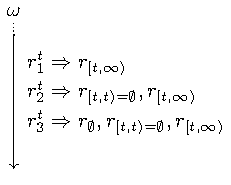
\includegraphics[width=0.4\textwidth]{figures/time-travel/empty-ranges} &
		\vspace{0pt} 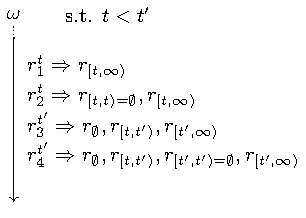
\includegraphics[width=0.44\textwidth]{figures/time-travel/empty-ranges-2} \\
		(a) & (b)
	\end{tabular}
	\caption{Two variations of the empty validity ranges issue occurring.}
	\label{fig:empty-ranges}
\end{figure}

When dealing with ranges, the fact that $\emptyset$ is indeed a valid range should be accounted for:
$$
\left[t, t\right) = \emptyset, \forall t \; .
$$

This has the inherent meaning, in our domain, that two different records for the same table were issued at the exact same time $t$.
Figure \ref{fig:empty-ranges} depicts the issue described in this Section, in two variations: (a) three records originated at the same instant $t$, and (b) four records were emitted at two different instants.

The issue that arises is the collision of primary keys; that is, the primary key of $r$ can be repeated multiple times, if all the relevant rows at the destination database have different validity ranges.

At first, this may seem an issue that could possibly be dismissed as very unlikely, since in order to occur it requires that records are emitted in the same moment.
Nevertheless, the presence of database transactions makes the significance of this scenario become evident.
Within a transaction, different queries are evaluated and later performed as a single atomic operation,\footnote{%
	From \cite[\S 6.6.3]{db-systems}:
	\begin{quote}
		A transaction is a collection of one or more operations on the database that must be executed atomically; that is, either all operations are performed or none are.
	\end{quote}
} thus resulting in several records being issued at the same instant; i.e. PostgreSQL writes several changes to the WAL within a single system call, and these changes may, and in certain cases do, contain multiple configurations of $r$.

The solution to this problem was a temporary one; that is, without any other alternatives being achievable in the internship time frame, it was decided to settle for the following solution.
Instead of using the record emission time, utilize the serialization time at the destination database.
In fact, using the database's system clock ensures a positive time drift.
Because the various operations are performed as transactions themselves, and they are not batched together,\footnote{%
	Cfr. \S \ref{sec:batching}.
} the small amount of time between the transactions is sufficient to prevent the problem presented in this Section.

A better solution is presented in \S \ref{sec:squashing-transactions}.


\subsection{Updates to Primary Keys}

An update to a time traveled primary key's value is effectively indistinguishable from the consecutive application of a deletion and a subsequent insertion;\footnote{%
	Conversely, a deletion and insertion would be indistinguishable from an update, if those two operations were performed inside a transaction, as discussed in the prior Section.
} that is, by following Operations (\ref{tt:insert}), (\ref{tt:update}), and (\ref{tt:delete}), one cannot distinguish between the two scenarios.

\begin{example}
	Table $\phi$'s primary key is a single string attribute \emph{id}.
	Row $q \in \phi$, with \emph{id} = ``Facco'', is updated to have \emph{id} = ``Fakko'', at instant $t$, without any issues from the data source's side.
	Following Operation (\ref{tt:update}), $q_{i-1}$ is updated to have its validity end in $t$, and $q_i$, containing the updated value for \emph{id}, is inserted with validity starting in $t$.
	
	There is no sensible mechanism that solely comprises an inquiry into the contents of $\dest{\phi}$, to tell whether at time $t$ an update operation was received for $q$, or rather a deletion request was received for $q$, in conjunction with an insertion request for a supposedly different row $q'$.
\end{example}

Of course, there is a semantic difference between an update and the operations described, even with regards to primary keys.
Nonetheless, it would not be possible to correlate distinct row configurations, if primary keys were not the driver for this correlation.

Though in the application that pertains to this Thesis updates to primary keys are voluntarily dismissed as not relevant to the use case at hand, it is important to note this limitation of the approach to time data described in this Chapter.


\subsection{Ignoring Unchanged Rows}

In developing this system, another issue arose: since time traveled tables are generally defined as a projection over some subset $S$ of the source table's columns, it is possible for a row to receive an update that contains the previous row configuration.
Formally,
$$
\dest{\omega} := \tau\big(\pi_{S}\big(\source{\omega}\big)\big) \Rightarrow
\text{it is possible that } \exists r, i \text{ s.t. } r_{i-1} = r_i \; .
$$

This is because when an update is performed in $\source{\omega}$, PostgreSQL writes the related data onto the WAL, which is in turn read by Debezium.
This process is carried out regardless of the fact that the updated value resides in a column that is not part of $S$, and if that is the case, the received record effectively asks to update a row to the configuration it already has.

When considering other tables, such as plain or aggregated tables, this problem can be trivially dismissed; that is, the update doesn't actually cause data in the output database to change.
Nevertheless, when considering time traveled tables, what happens is that the row will be repeated with two validity ranges, the former ending in some instant $t$ and the latter beginning at $t$.

Thus, while querying the output database one would be induced to think that since the two validity ranges represent a change, then the row was changed, which is not actually the case.

Although this behavior does not in fact go against Definition (\ref{def:tau}), the relatively diminished semantic significance of the validity range concept, as well as the inefficiency it entails, were sufficient reasons to develop a guarding mechanism against what effectively becomes an unnecessary duplication of data.

This guard can be found in Listing \ref{src:eu.spaziodati.metrics/connectors/PostgresSinkTask.scala}, lines 72 -- 76: the \texttt{NOT EXISTS} SQL clause is used to check whether, as previously expressed, $r_{i-1} = r_i$.
